\documentclass[11pt,a4paper,oneside,titlepage]{article}
\usepackage[utf8]{inputenc}
\usepackage{amsmath}
\usepackage{amsfonts}
\usepackage{amssymb}
\usepackage{graphicx}
\usepackage{minitoc}
\usepackage{xcolor, textcomp}
\usepackage{siunitx}

\usepackage{tikz}
\usetikzlibrary{trees}


\author{Matteo Busi}
\title{SPM Final Project Report}

\newcommand{\HRule}{\rule{\linewidth}{0.5mm}} % Defines a new command for the horizontal lines, change thickness here
\newcommand{\HRuleL}{\rule{1.1\linewidth}{0.5mm}} % Defines a new command for the horizontal lines, change thickness here

\usepackage{listings}
\usepackage[]{algorithm2e}


\definecolor{listinggray}{gray}{0.9}
\definecolor{lbcolor}{rgb}{0.9,0.9,0.9}
\lstset{
	backgroundcolor=\color{lbcolor},
	language=C++,
	breaklines=true,
	identifierstyle=\textbf\ttfamily,
	basicstyle=\ttfamily\small,
	tabsize=4,
	captionpos=b,
}

\newcommand{\alert}[1]{{\color{red}#1}}

\begin{document}
	
	\begin{titlepage}
				
		\center % Center everything on the page
		
		%----------------------------------------------------------------------------------------
		%	HEADING SECTIONS
		%----------------------------------------------------------------------------------------
		
		\textsc{\LARGE Universit\`a di Pisa}\\[1.5cm] % Name of your university/college
		\textsc{\Large Department of Computer Science}\\[1.5cm] % Major heading such as course name
		%\textsc{\large SPM Final Project Report}\\[0.5cm] % Minor heading such as course title
		
		%----------------------------------------------------------------------------------------
		%	TITLE SECTION
		%----------------------------------------------------------------------------------------
		
		\HRule \\[1cm]
		{ \huge \bfseries SPM Final Project Report}\\[0.4cm] % Title of your document
		{ \Large The Jacobi Iterative Method }\\[0.4cm]
		\HRule \\[1.5cm]
		
		%----------------------------------------------------------------------------------------
		%	AUTHOR SECTION
		%----------------------------------------------------------------------------------------
		
%		\begin{minipage}{0.4\textwidth}
%			\begin{flushleft} \large
%				\emph{Author:}\\
%				Matteo \textsc{Busi} % Your name
%			\end{flushleft}
%		\end{minipage}
%		~
%		\begin{minipage}{0.4\textwidth}
%			\begin{flushright} \large
%				\emph{Supervisor:} \\
%				Dr. James \textsc{Smith} % Supervisor's Name
%			\end{flushright}
%		\end{minipage}\\[2cm]
		
		% If you don't want a supervisor, uncomment the two lines below and remove the section above
		\Large %\emph{Author:}\\
		\textsc{Matteo Busi}\\[0.4cm]% Your name
		\large
		\textsc{Student ID. 494087}\\[3cm]
		
		%----------------------------------------------------------------------------------------
		%	DATE SECTION
		%----------------------------------------------------------------------------------------
		
		{\large \today}\\[2cm] % Date, change the \today to a set date if you want to be precise
		
		%----------------------------------------------------------------------------------------
		%	LOGO SECTION
		%----------------------------------------------------------------------------------------
		
		%\includegraphics{logo.png}\\[1cm] % Include a department/university logo - this will require the graphicx package
		
		%----------------------------------------------------------------------------------------
		
		\vfill % Fill the rest of the page with whitespace
		
	\end{titlepage}

	\section{Introduction} \label{sec:intro}
		The aim of this project was to produce a program to solve linear systems using the Jacobi method.

Three different implementations are proposed here:
\begin{description}
    \item[Sequential implementation] the sequential implementation provides a \\    
    vanilla implementation of the Jacobi method,
    \item[Thread implementation] is a na\"ive implementation of the algorithm using \lstinline+thread+s from \lstinline|C++11| standard,  
    \item[FastFlow implementation] is an implementation using the \lstinline+parallelFor+ from FastFlow library.
\end{description}

Tests were conducted on a machine using a \emph{Intel Xeon E2650} CPU ($8$ cores clocked at $2$~\si{\giga\hertz} each with $2$ contexts) and a \emph{Intel Xeon Phi} co-processor ($60$ cores clocked at $1$~\si{\giga\hertz} each with $4$ contexts).

\paragraph{Summary.} The next section discusses the details of program design, including an analysis of the expected performance of the sequential and parallel implementations.
Section~\ref{sec:implementation} reports some details about the implementation, discussing the classes design, their methods, and some optimization.
\alert{Section~\ref{sec:experiments} is divided in two sub-sections. 
The first sub-section discusses the methodology for the experiments and chosen parameters, while the second sub-section reports the experimental results in the form of tables and graphs.
Section~\ref{sec:guide} includes the user manual for the program, and indications on how to reproduce results reported here.
Finally Section~\ref{sec:conclusions} compares obtained results against the expected ones.}
		
	\section{Design} \label{sec:design}
		In this section the basic Jacobi algorithm is introduced.
Then a brief account on design choices, driven by the performance model, is given along with a sketch of the parallel algorithm.

\subsection{Sequential algorithm and performance}\label{subsec:seq}
Figure~\ref{alg:sequantialjacobi} shows the pseudo-code for the Jacobi iterative method as presented in the numerical computing literature~\cite{}.
\begin{figure}[h]
	\begin{center}
	\begin{algorithm}[H]
		\KwData{A linear system in the form of $Ax = b$ with $N \times N$ the size of $A$, a maximum accepted error $\varepsilon$, and a maximum number of iterations $K$.}
		\KwResult{An approximated solution $x^{(k)}$ s.t. $||b - Ax^{(k)}||^{2}_2 \leq \varepsilon$ or $k \ge K$.}
		\BlankLine
		$x^{(0)} \leftarrow $ initial guess for the solution\\
		$k \leftarrow 0$\\
		\While {$||b - Ax^{(k)}||^{2}_2 \ge \varepsilon$ and $k \leq K$}
		{
			\For{$i\leftarrow 0$ \KwTo $N$}{
				$\sigma \leftarrow 0$\\
				\For{$j\leftarrow 0$ \KwTo $N$}{
					\If{$j \neq i$}{
						$\sigma$ $\leftarrow$ $\sigma + a_{ij}x^{(k)}_j$
					}
				}
				$x^{(k+1)}_i \leftarrow \frac{b_i - \sigma}{a_{ii}}$\\
			}
			$k \leftarrow k + 1$\\
		}
	\end{algorithm}
	\end{center}
	\caption{Pseudo-code for the sequential Jacobi iterative method.}
	\label{alg:sequantialjacobi}
\end{figure}

It is pretty evident that the completion time $T_C$ for a program using this procedure could be computed as:
\[
	T_C = T_{alloc}(n) + T_{fill}(n) + T_{jacobi}(n)
\]

where $T_{alloc}(n)$ and $T_{fill}(n)$ are, respectively, the time needed do allocate and fill the memory to store the input data, and $T_{jacobi}(n)$ is the time to solve the system using the algorithm in Figure~\ref{alg:sequantialjacobi} (i.e.\ the latency).

Further expanding $T_{jacobi}$ we get:
\[
	T_{jacobi}(n) = k \cdot (T_{conv}(n) + T_{comp}(n) + T_{upd}(n))
\]
where $T_{conv}(n)$ is the time needed to check convergence, $T_{comp}(n)$ is the time needed to compute the new approximation of the solution, and $T_{upd}(n)$ is the time needed to update the solution vector.

Basic complexity theory allow us to conclude that $T_{conv}(n)$ and $T_{upd}(n)$ have linear complexity and $T_{comp}(n)$'s complexity is quadratic.
It is worth, then, to parallelize the computation corresponding to time $T_{comp}(n)$ (i.e.\ the computation of the new value of $x$).

\subsection{Parallel algorithm and performance}\label{subsec:par}
Observations of the previous sub-section let us to design a worker.
The idea is to split the matrix $A$ in rows of the same size and to feed said rows to the worker.

The performance model depends also on the number of workers, $w$, and $ T_{jacobi}(n, w)$ can be expanded --- ignoring $T_{conv}(n)$ and $T_{upd}(n)$ --- as:
\[
	 T_{jacobi}(n, w) = T_{setup} (n, w) + T_{barrier} (n, w) + \frac{k}{w} \cdot T_{comp}(n)
\]
where $T_{setup} (n, w)$ is the time required to setup the $w$ workers, $T_{barrier} (n, w)$ is the total time spent by threads waiting each other and $\frac{k}{w} \cdot T_{comp}(n)$ is the ideal time needed to $w$ workers to compute the new value of the approximation of the solution.
		
	\section{Implementation} \label{sec:implementation}
		The actual implementation consists in three different variants of the Jacobi iterative method, following the ideas in Section~\ref{sec:design}.

The source code is organized as follows:
\begin{itemize}
	\item The main function, in file \verb|main.cpp|, implements the parameter parsing, I/O and initialization.
	\item The class \verb|JacobiReport| collects statistics about the execution of the algorithm.
	\item The class \verb|JacobiSolver| that implements, together with class \verb|JacobiSequentialSolver|, \verb|JacobiFFSolver|, and \verb|JacobiThreadSolver| a template method pattern.
	Each of the concrete sub-classes implement a \verb|deltax| method specifying how the new approximation of the solution $x$ to the system is computed.
	\item Class \verb|JacobiSequentialSolver| implements \verb|deltax| exactly as in Algorithm~\ref{alg:sequantialjacobi}
	\item Class \verb|JacobiFFSolver| implements \verb|deltax| using the \verb|parallel_for| building block from FastFlow library; \verb|parallel_for| automatically parallelizes the given loop.
	\item Class \verb|JacobiThreadSolver| implements \verb|deltax| using C++ threads. The implementation is na\"ive, meaning that the threads are re-created at each method invocation (i.e.\ $T_{setup}$ may become non negligible)  and the collector is a simple barrier implemented using \verb|join| method from \verb|thread| class.
\end{itemize}

Please note that, the code of each \verb|deltax| (and also other methods) have been made vectorizable using the feedback provided by the compiler.
Specifically the \verb|if| construct present in the inner-loop in the algorithms above have been removed and the loop have been split in two parts, i.e.\ the first part in range $[0, i)$ and the second $[i+1, N)$ (or  $[i+1, M)$ in case of parallel implementation).
			
	\section{Experiments} \label{sec:experiments}
		This section summarizes how the experiments were conducted and their results.

\subsection{Methodology} \label{subsec:methodology}
Experiments are performed using the script \verb|jacobirun.sh|, as better explained in sub-section~\ref{subsec:runningexperiments}.
The script runs sequential, thread and FastFlow versions both on the Xeon CPU and Xeon Phi co-processor.
If on the Xeon CPU The number of workers for parallel versions goes from $1$ to $16$, otherwise it ranges from $1$ to $240$ (to match the number of threads of each processor).
$N$, instead, assumes values of $5000$, $10000$, $15000$, and $30000$. Sadly bigger values of $N$ quickly filled up the memory of the co-processor, hence they were not included in the analysis.
All the tests of the FastFlow implementation use a grain size of $10$.

\subsection{Results and remarks} \label{subsec:results}
Each of the graphs in this section reports experimental results in terms of efficiency, scalability, and speedup of each experiment described above.
\begin{figure}
	\centering
	\begin{subfigure}[b]{0.3\linewidth}
		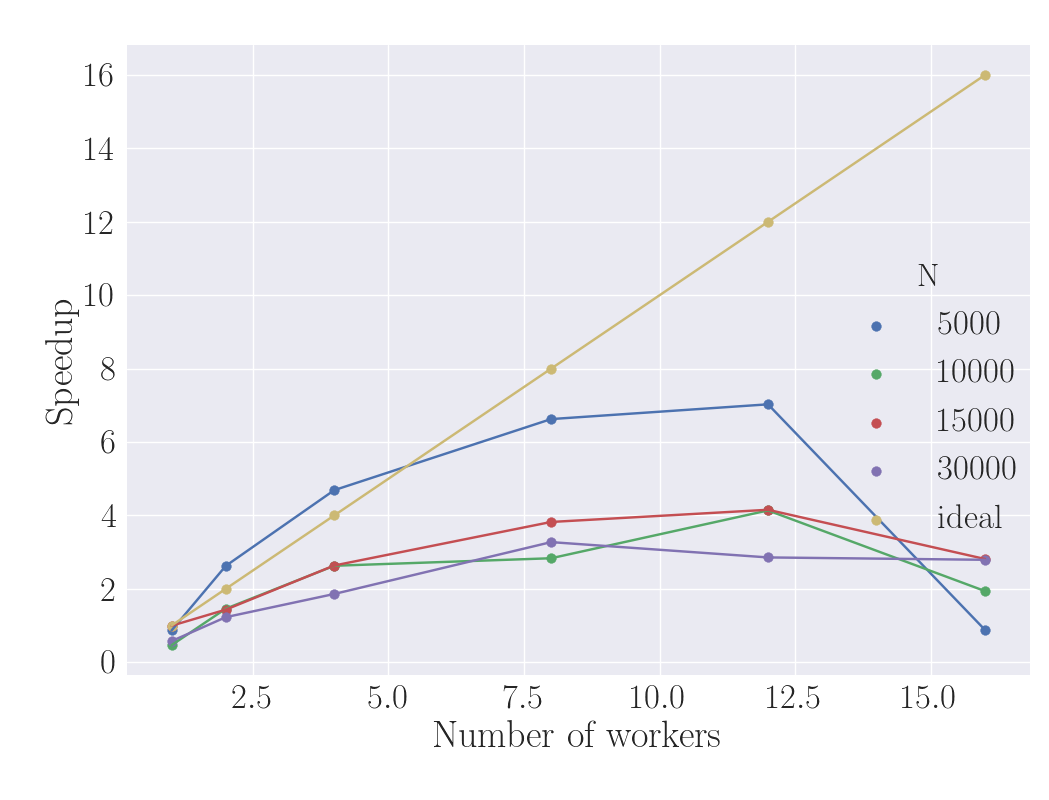
\includegraphics[width=\linewidth]{../graphs/graph_ff_host_s}
		\caption{Speedup graph.}
		\label{fig:ff_host_s}
	\end{subfigure}
	\begin{subfigure}[b]{0.3\linewidth}
		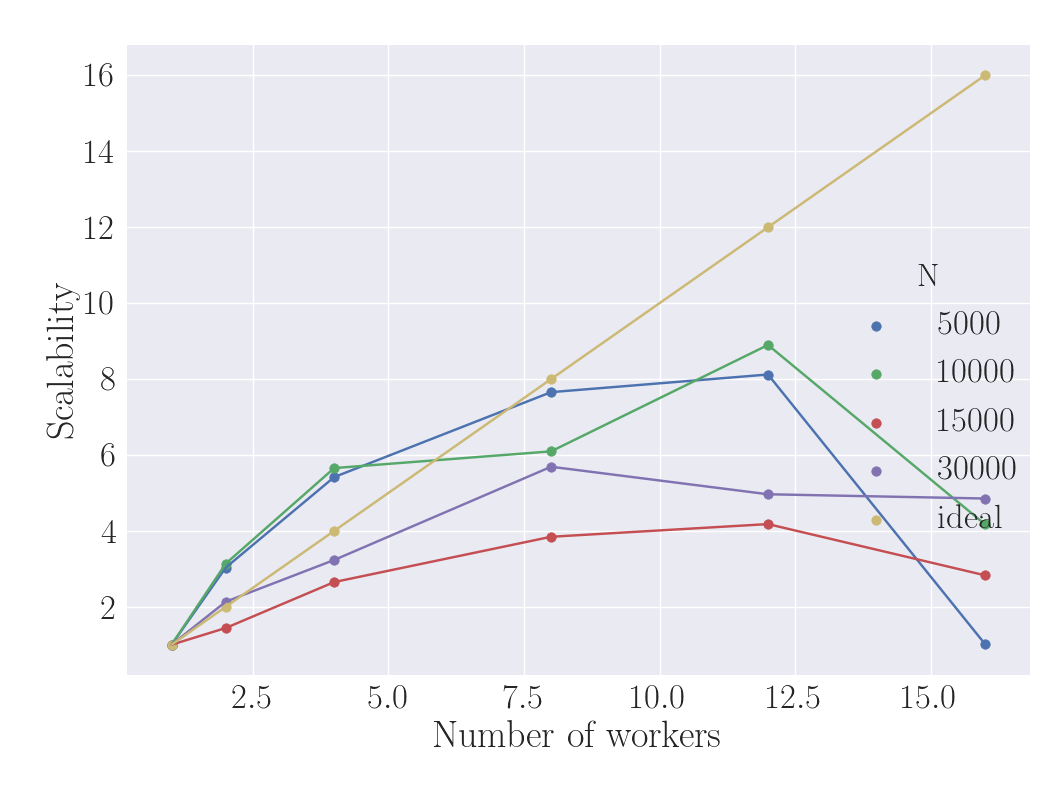
\includegraphics[width=\linewidth]{../graphs/graph_ff_host_scalab}
		\caption{Scalability graph}
		\label{fig:ff_host_scalab}
	\end{subfigure}
	\begin{subfigure}[b]{0.3\linewidth}
		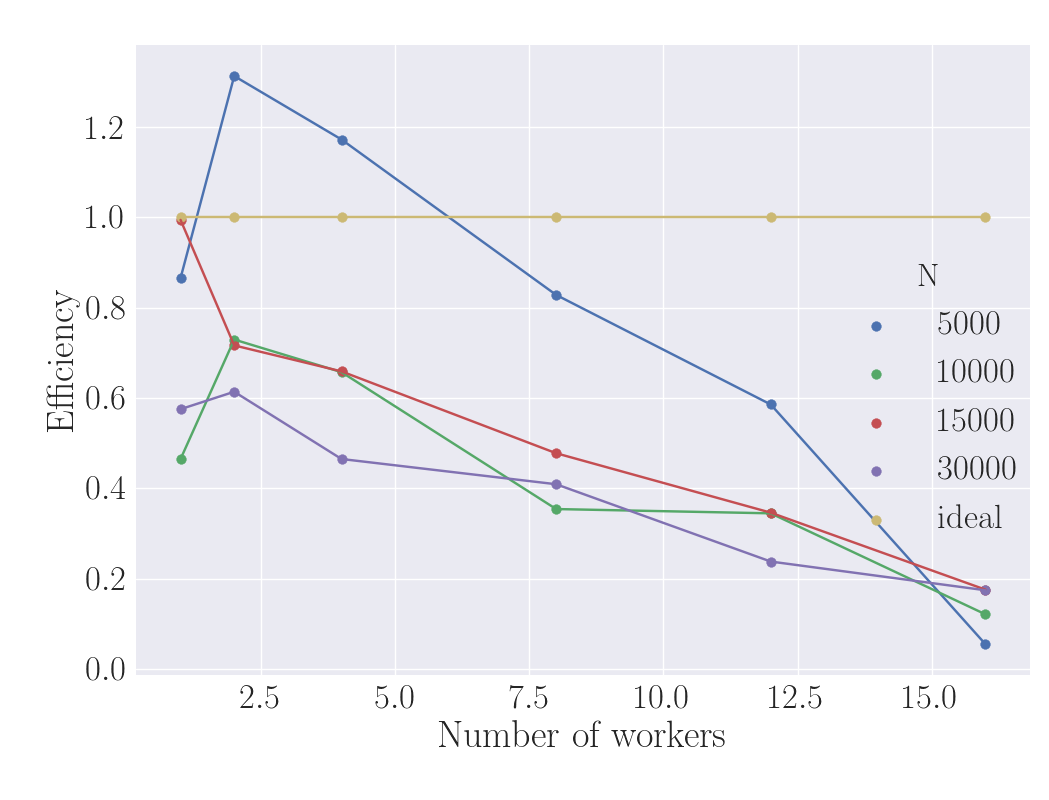
\includegraphics[width=\linewidth]{../graphs/graph_ff_host_eff}
		\caption{Efficiency graph}
		\label{fig:ff_host_eff}
	\end{subfigure}
	\caption{Graphs of different performance measures for $N \in \{5000, 10000, 15000, 30000\}$ on the Xeon CPU using FastFlow}
	\label{fig:ff_host}
\end{figure}
\begin{figure}
	\centering
	\begin{subfigure}[b]{0.3\textwidth}
		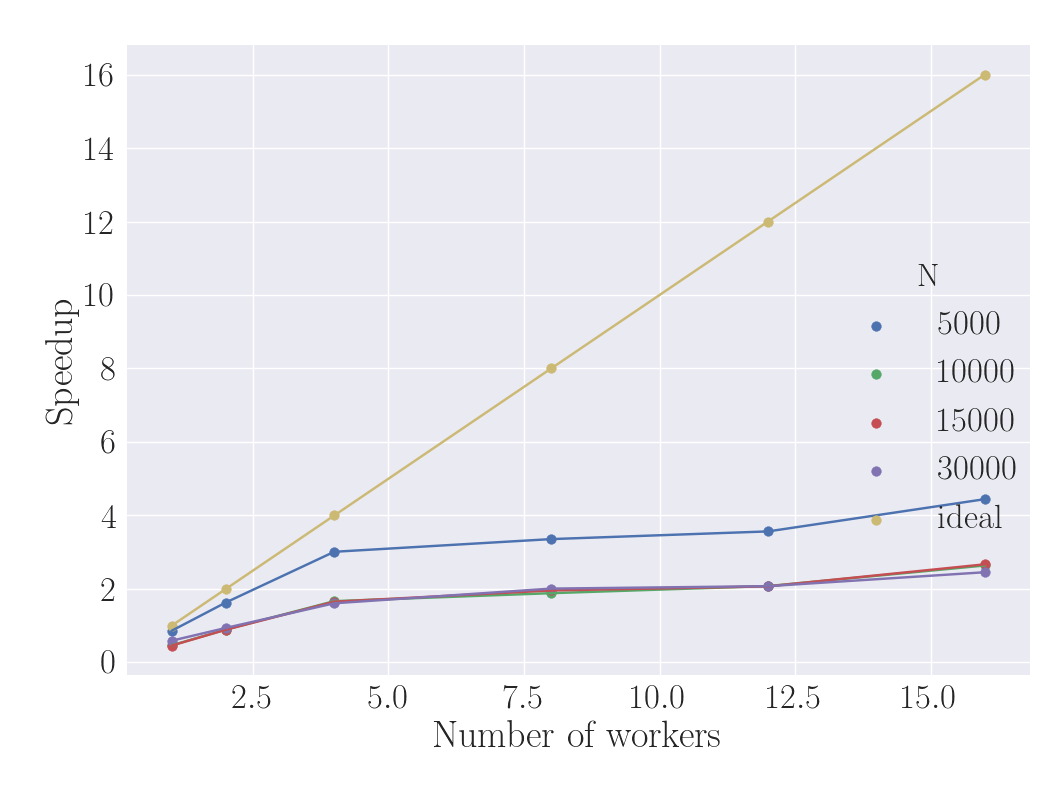
\includegraphics[width=\textwidth]{../graphs/graph_th_host_s}
		\caption{Speedup graph.}
		\label{fig:th_host_s}
	\end{subfigure}
	\begin{subfigure}[b]{0.3\textwidth}
		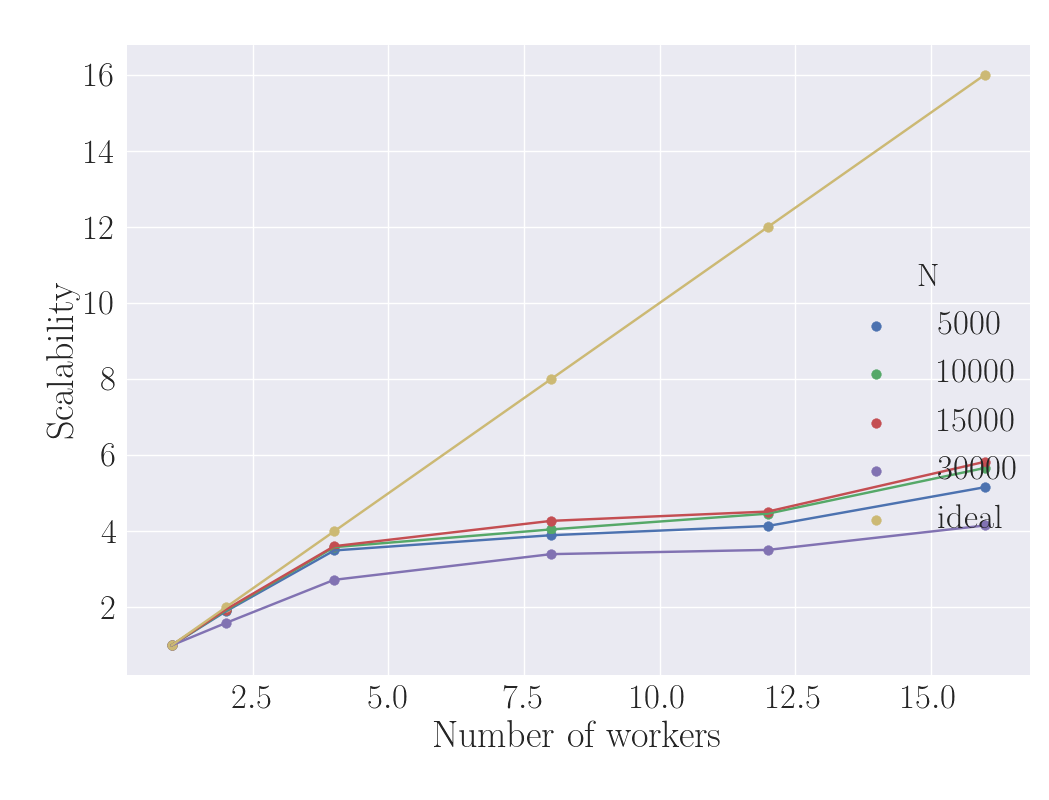
\includegraphics[width=\textwidth]{../graphs/graph_th_host_scalab}
		\caption{Scalability graph}
		\label{fig:th_host_scalab}
	\end{subfigure}
	\begin{subfigure}[b]{0.3\textwidth}
		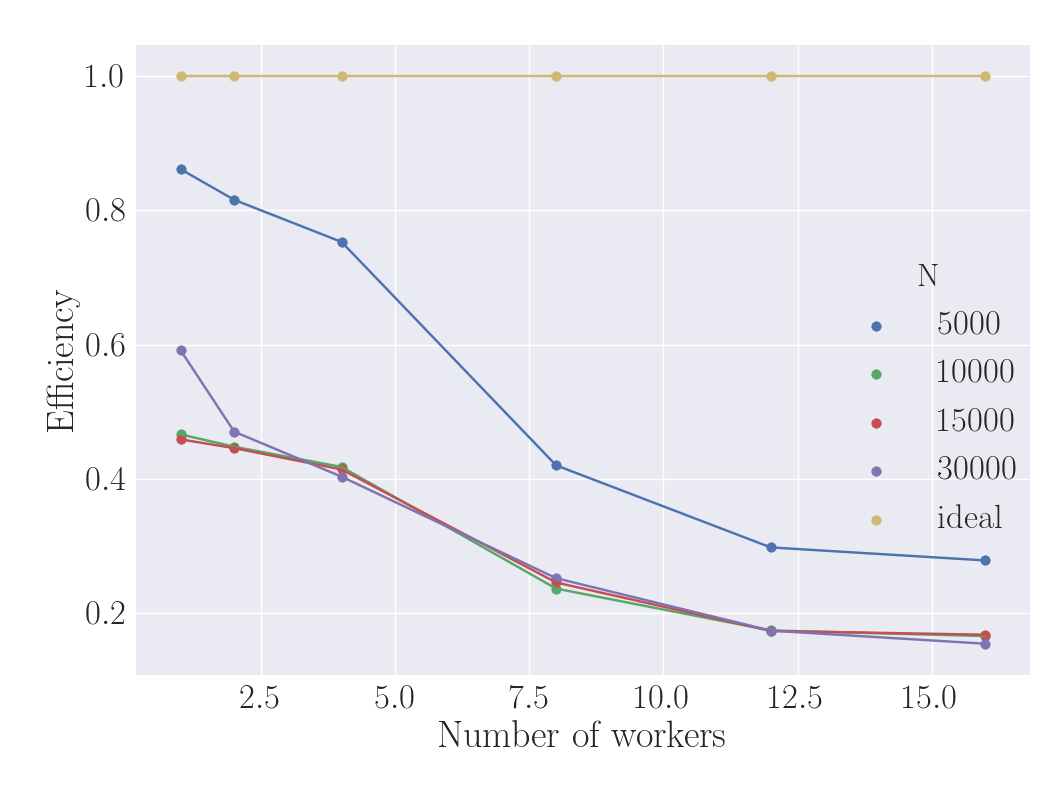
\includegraphics[width=\textwidth]{../graphs/graph_th_host_eff}
		\caption{Efficiency graph}
		\label{fig:th_host_eff}
	\end{subfigure}
	\caption{Graphs of different performance measures for $N \in \{5000, 10000, 15000, 30000\}$ on the Xeon CPU using C++11 threads}
	\label{fig:th_host}
\end{figure}
Figure~\ref{fig:ff_host} and Figure~\ref{fig:th_host} respectively report the results of the execution of the FastFlow and C++11 thread implementation on the Xeon CPU.
It is interesting to see that none of the measured metrics adhere to the ideal curve, especially for bigger $N$s.
Smaller $N$s lead to better performance metrics, probably this is partly due to the time spent in barrier and in the setup of the workers and partly due to the time spent by the processor in performing cache coherence.
\begin{figure}
	\centering
	\begin{subfigure}[b]{0.3\textwidth}
		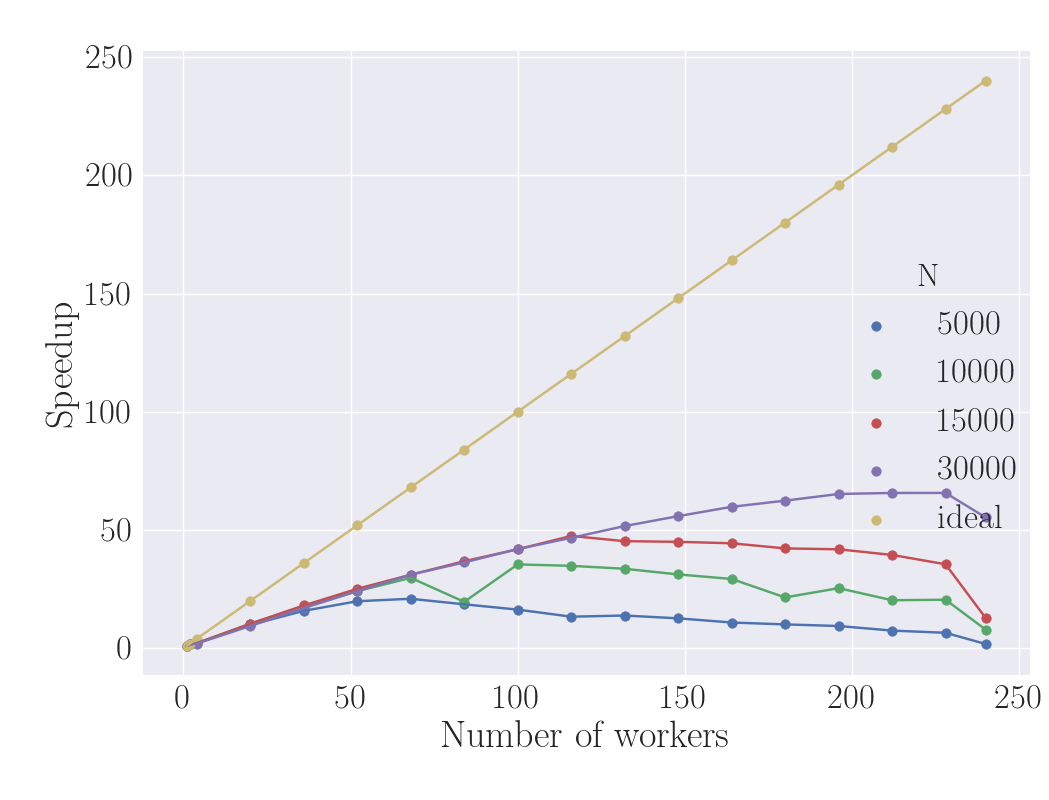
\includegraphics[width=\textwidth]{../graphs/graph_ff_mic_s}
		\caption{Speedup graph.}
		\label{fig:ff_mic_s}
	\end{subfigure}
	\begin{subfigure}[b]{0.3\textwidth}
		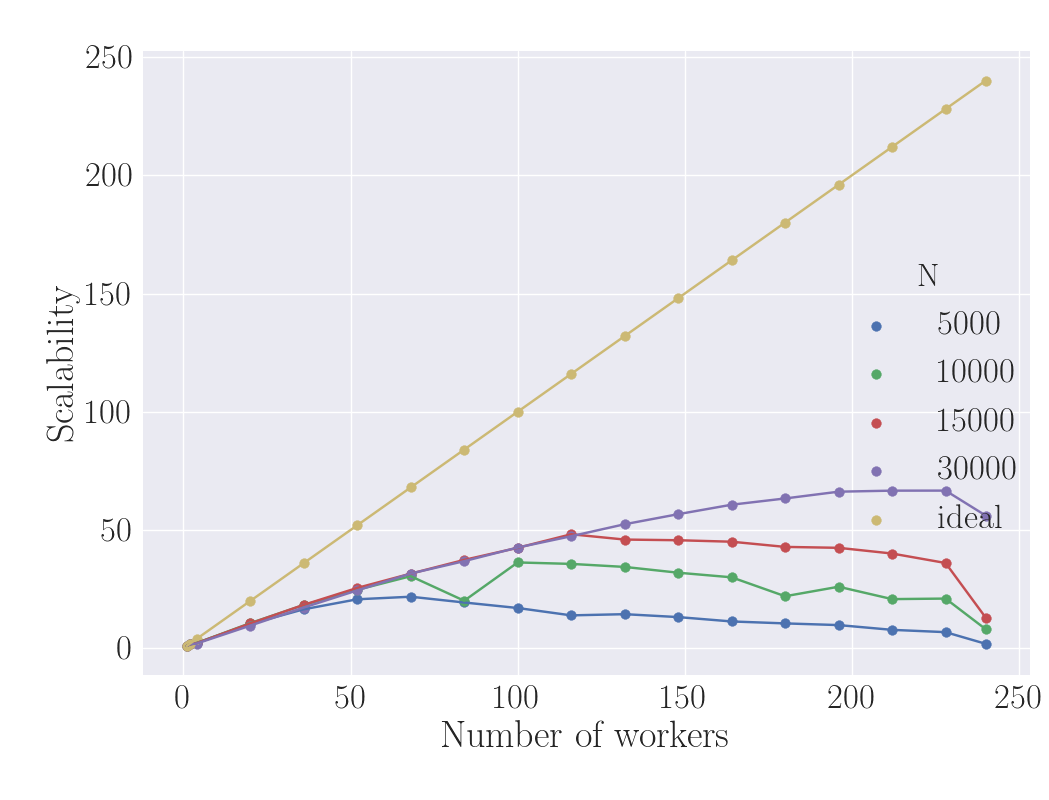
\includegraphics[width=\textwidth]{../graphs/graph_ff_mic_scalab}
		\caption{Scalability graph}
		\label{fig:ff_mic_scalab}
	\end{subfigure}
	\begin{subfigure}[b]{0.3\textwidth}
		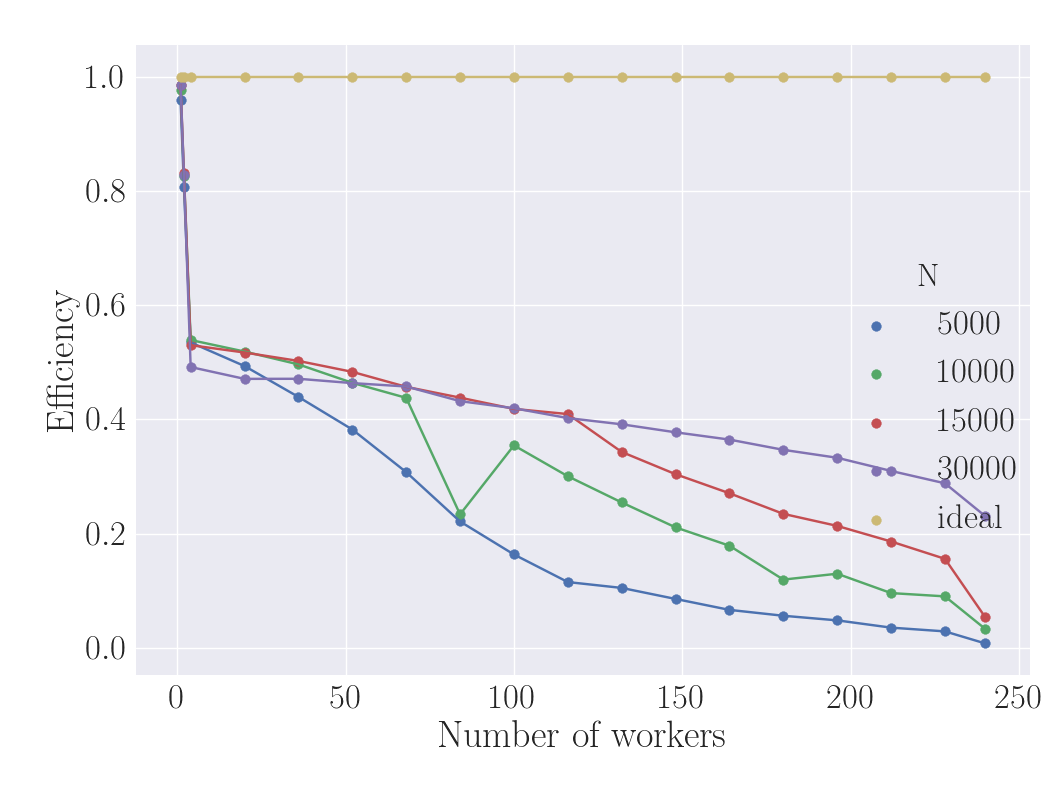
\includegraphics[width=\textwidth]{../graphs/graph_ff_mic_eff}
		\caption{Efficiency graph}
		\label{fig:ff_mic_eff}
	\end{subfigure}
	\caption{Graphs of different performance measures for $N \in \{5000, 10000, 15000, 30000\}$ on the Xeon Phi co-processor using FastFlow}
	\label{fig:ff_mic}
\end{figure}
\begin{figure}
	\centering
	\begin{subfigure}[b]{0.3\textwidth}
		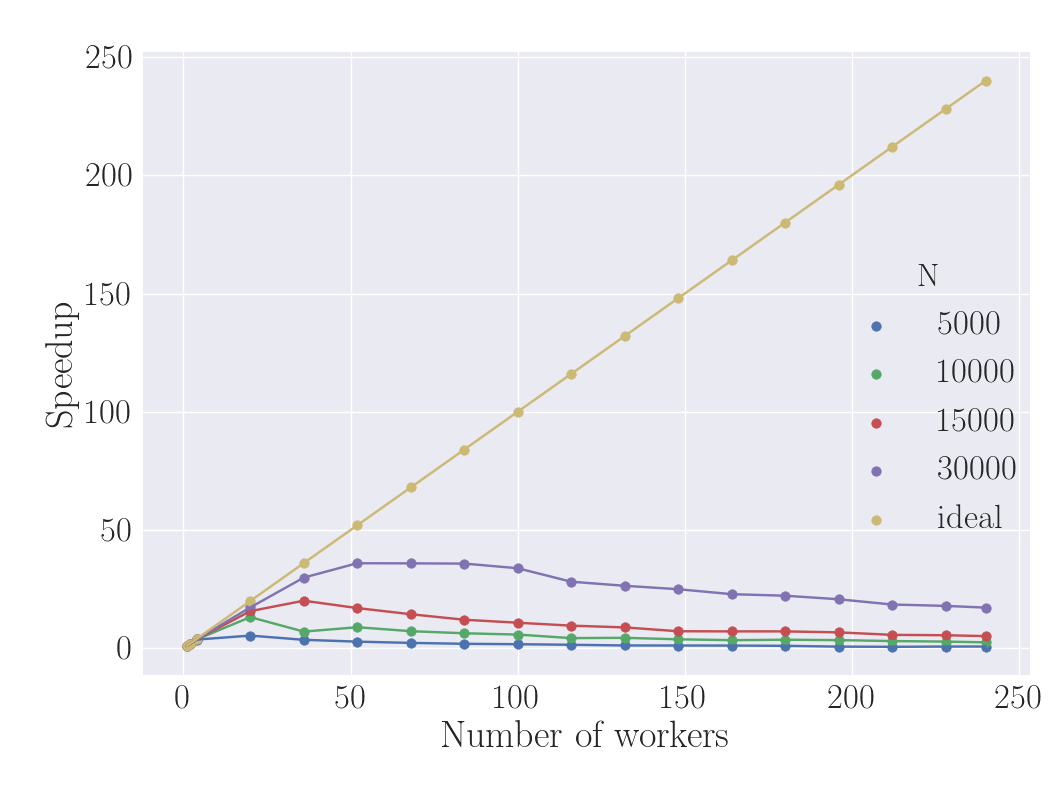
\includegraphics[width=\textwidth]{../graphs/graph_th_mic_s}
		\caption{Speedup graph.}
		\label{fig:th_mic_s}
	\end{subfigure}
	\begin{subfigure}[b]{0.3\textwidth}
		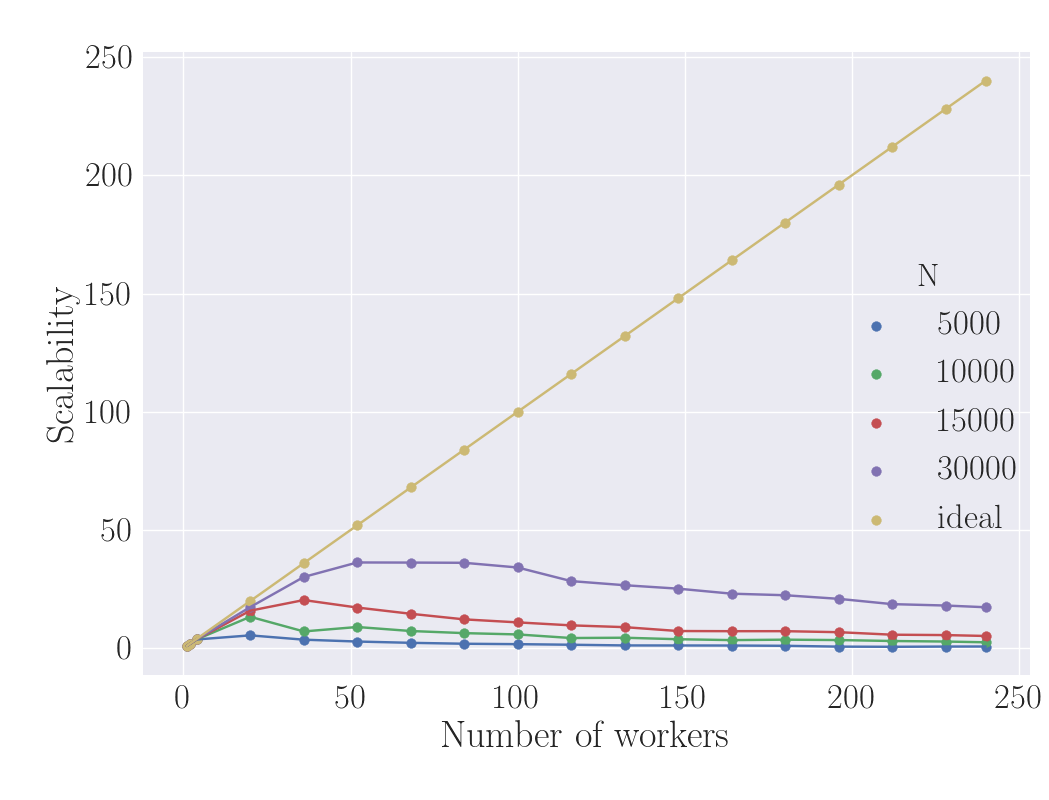
\includegraphics[width=\textwidth]{../graphs/graph_th_mic_scalab}
		\caption{Scalability graph}
		\label{fig:th_mic_scalab}
	\end{subfigure}
	\begin{subfigure}[b]{0.3\textwidth}
		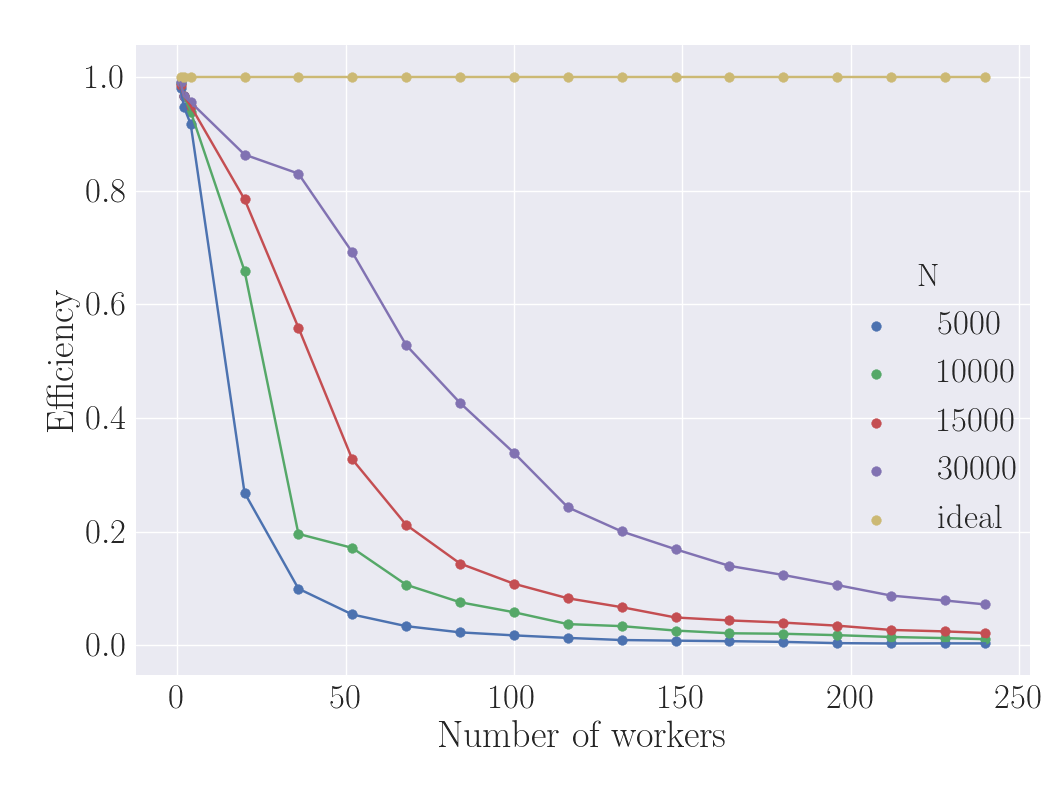
\includegraphics[width=\textwidth]{../graphs/graph_th_mic_eff}
		\caption{Efficiency graph}
		\label{fig:th_mic_eff}
	\end{subfigure}
	\caption{Graphs of different performance measures for $N \in \{5000, 10000, 15000, 30000\}$ on the Xeon Phi co-processor using C++11 threads}
	\label{fig:th_mic}
\end{figure}
Figure~\ref{fig:ff_mic} and Figure~\ref{fig:th_mic} respectively report the results of the execution of the FastFlow and C++11 thread implementation on the Xeon Phi co-processor.
As above none of the measured metrics adhere to the ideal curve.
In this case, on the other hand, bigger $N$s lead to better performance metrics since the time spent in barrier and in the setup of the workers becomes smaller w.r.t.\ effective time of computation.
In this case (up to $N = 30000$) cache coherence probably is not a bottleneck, since the cache on the Xeon Phi is bigger than the one on the Xeon CPU.
\begin{table}
	\centering
	\begin{tabular}{llr}  
		\toprule
		\multicolumn{2}{c}{Item} \\
		\cmidrule(r){1-2}
		Animal    & Description & Price (\$) \\
		\midrule
		Gnat      & per gram    & 13.65      \\
		&    each     & 0.01       \\
		Gnu       & stuffed     & 92.50      \\
		Emu       & stuffed     & 33.33      \\
		Armadillo & frozen      & 8.99       \\
		\bottomrule
	\end{tabular}
	\caption{Best configurations in terms of minimal latency for FastFlow implementation at different values of $N$}
	\label{tab:ff}
\end{table}
~
\begin{table}
	\centering
	\begin{tabular}{llr}  
		\toprule
		\multicolumn{2}{c}{Item} \\
		\cmidrule(r){1-2}
		Animal    & Description & Price (\$) \\
		\midrule
		Gnat      & per gram    & 13.65      \\
		&    each     & 0.01       \\
		Gnu       & stuffed     & 92.50      \\
		Emu       & stuffed     & 33.33      \\
		Armadillo & frozen      & 8.99       \\
		\bottomrule
	\end{tabular}
	\caption{Best configurations in terms of minimal latency for C++11 thread implementation at different values of $N$}
	\label{tab:th}
\end{table}
Table~\ref{tab:ff} shows, for each size $N$ of the system, the best configuration in terms of latency for the FastFlow implementation.
Table~\ref{tab:th} shows the same data as Table~\ref{tab:ff}, but reports also the ratio between setup/barrier time and computing time (i.e.\ $({T_{barrier} + T_{setup})/T_{comp}}$) (full data is available in folder \verb|results| as \verb|csv| file, as explained in Section~\ref{sec:guide}).

Please note that (almost) none of the best configurations include a number of workers equal to the number of contexts, this is due to the fact that usually at least one context is used for orchestration.

	
	\section{User guide} \label{sec:guide}
		This section provides a short guide on how to use the program, how to conduct the experiments, and how to gather the results.

\subsection{Workspace}
The workspace content is organized as follows:
\begin{itemize}
	\item The folder \verb|bin| contains the results of the compilation (including vectorization reports),
	\item the folder \verb|graphs| contains the graphs generated by \verb|reportgen.py|,
	\item the folder \verb|results| contains the collection of \verb|csv| files generated by \verb|jacobirun.sh|,
	\item the folder \verb|src| contains the source code of the program,
	\item the bash script \verb|jacobirun.sh| contains the code to run experiments,
	\item the Python program \verb|reportgen.py| that generates graphs starting from data in \verb|results| folder,
	\item the make file \verb|Makefile| compiles the project as explained in sub-section~\ref{subsec:compilation}.
\end{itemize}

In the following we assume that the current working directory is the root of the workspace.

\subsection{Compilation}\label{subsec:compilation}
To compile the project a \verb|Makefile| with four rules is provided:
\begin{enumerate}
	\item Executing \verb|make jacobix| the executable for the Xeon CPU is produced and placed in \verb|bin/jacobix|,
	\item executing \verb|make jacobim| the executable for the Xeon Phi is produced and placed in \verb|bin/jacobim|,
	\item executing \verb|make offload| the executable for the Xeon Phi is produced and placed in both \verb|bin/jacobim| and in the home directory on \verb|mic1|,
	\item executing \verb|make clean| the files produced by compilation, testing, and analysis are deleted.
\end{enumerate}

\subsection{Program usage}
To run a single resolution of a random system one of the compiled executables located in \verb|bin| must be run.
Executable \verb|jacobix| runs on the Xeon CPU, while executable \verb|jacobim| must be offloaded to the Xeon Phi.

Executing one of the executable without arguments produces as output a guide that should be self-explaining:
\begin{lstlisting}
Usage: bin/jacobix N ITER ERR METHOD [NWORKERS] [GRAIN]
Where: 
N : is the size of the matrix A
ITER : is the maximum number of iterations
ERR : is the maximum norm of an acceptable error
METHOD: is either
	s : indicating that the sequential implementation must be used
	f : indicating that the FastFlow implementation must be used
	t : indicating that the Thread implementation must be used
NWORKERS : the number of workers that should be used (ignored if METHOD is 's')
GRAIN : the grain of the computation (only if METHOD is 'f')

Produces a CSV line, in the form:
	N_WORKERS, N_ITERATIONS, COMP_TIME, UPD_TIME, CONV_TIME, SETUP_AND_BARRIER_TIME, LATENCY, ERROR
Where:
N_WORKERS : is the number of workers used
N_ITERATIONS : is the effective number of iterations performed
COMP_TIME : is the total time spent in computation of the new approximation
UPD_TIME : is the total time spent in updating the solution vector
CONV_TIME : is the total time spent in convergence checks
SETUP_AND_BARRIER_TIME : is the total time spent setting up threads and in barrier (computed only if METHOD is 't')
LATENCY : is the latency
ERROR : is norm of the error
\end{lstlisting}

\subsection{Experiments and analysis}\label{subsec:runningexperiments}
After compilation, to execute the experiments and analyse the results one must:
\begin{enumerate}
	\item run \verb|./jacobirun.sh| or \verb|./jacobirun.sh MIC| (if Xeon Phi must be used), 
	\item run \verb|reportgen.py| to produce graphs.
\end{enumerate}
	
	\section{Conclusion} \label{sec:conclusions}
		Summing up the data let us to conclude that:
\begin{itemize}
	\item The time spent in setting up the workers and in the barrier are not always negligible, especially for bigger $N$s
	\item On the other hand the ratio of time spent in setup increases as $w$ increases with small $N$s 
	\item Huge systems may not perform well since cache coherence procedures may spend non negligible time in moving data (i.e. incrementing the time for updating)
	\item Moreover small workloads in combination with \emph{vectorization} --- which dramatically improves the computation time increasing --- increase, again, the setup/barrier time fraction.
\end{itemize}

So, decent performances were achieved but to have better metrics one should, for example:
\begin{itemize}
	\item Optimize the code to work better on a specific architecture
	\item removing unnecessary memory allocations or use better allocators
	\item reduce idle time of each worker by giving a more evenly distributed workload
\end{itemize} 
	\bibliography{references}
\end{document}